\chapter{Problem Definition and Approach}
\label{chapter:problem-definition}
%% ======================================================================
%%  CME4150 Managing Uncertainty & Data - Team Challenge
%%  Strategic programming of maintenance, strengthening and replacement
%%  of quay walls in the Municipality of Utrecht.
%%
%%  Each section below is evaluated INDEPENDENTLY by a different teacher.
%%  Make every section self-explanatory and refer back to earlier
%%  sections where needed. Text beyond the page limit is NOT assessed.
%% ======================================================================

\section{Problem Synthesis and Goal Definition}
\label{sec:problem-synthesis}

%% ----------------------------------------------------------------------
%%  MAX 0.5 PAGE  |  RUBRIC WEIGHT 5%
%%
%%  TASK DESCRIPTION
%%  Define the scope of your problem and the specific goal(s). Considering
%%  your specific scope, analyse the main sources of uncertainty that
%%  should be considered in the analysis. You may focus on the most
%%  relevant ones that may affect the project progress and thus have a
%%  larger impact on the results. Justify your choices.
%%
%%  CHECKLIST (challenge task 1: scope the problem and name the dominant
%%  uncertainties)
%%   - Choose the assets you analyse: a designated stretch (a section of
%%     the inner-city canals, a stretch along the Vecht, the Vaartsche
%%     Rijn or the Leidsche Rijn, or a bank of the Merwedekanaal) or a
%%     portfolio-level analysis covering several stretches.
%%   - Describe structural typologies, approximate age and construction,
%%     the loads carried and the functions served: retaining ground and
%%     street, carrying traffic and trees, mooring and navigation, water
%%     level and water quality, heritage value, ecology.
%%   - Draw the system boundary explicitly. Does a privately owned wharf
%%     cellar belong to your system? Does the road on top, and the cable
%%     duct inside it?
%%   - Classify the uncertainties and argue which the municipality could
%%     actually reduce, at which temporal and economic cost, and which it
%%     must simply carry.
%%   - State the decision variable precisely: when to intervene, where to
%%     intervene first, how much to inspect, or how fast to spend. These
%%     are different problems with different answers.
%%   - State the decision horizon and the regulatory and institutional
%%     instruments that genuinely constrain the decision.
%%   - Map the stakeholders whose objectives conflict (residents,
%%     businesses, cellar owners, heritage authority, water authority,
%%     cyclists, freight) and note which conflicts your analysis will and
%%     will not resolve.
%% ----------------------------------------------------------------------


\begin{wrapfigure}{r}{7.0cm}
    \vspace{-8pt}
    \centering
    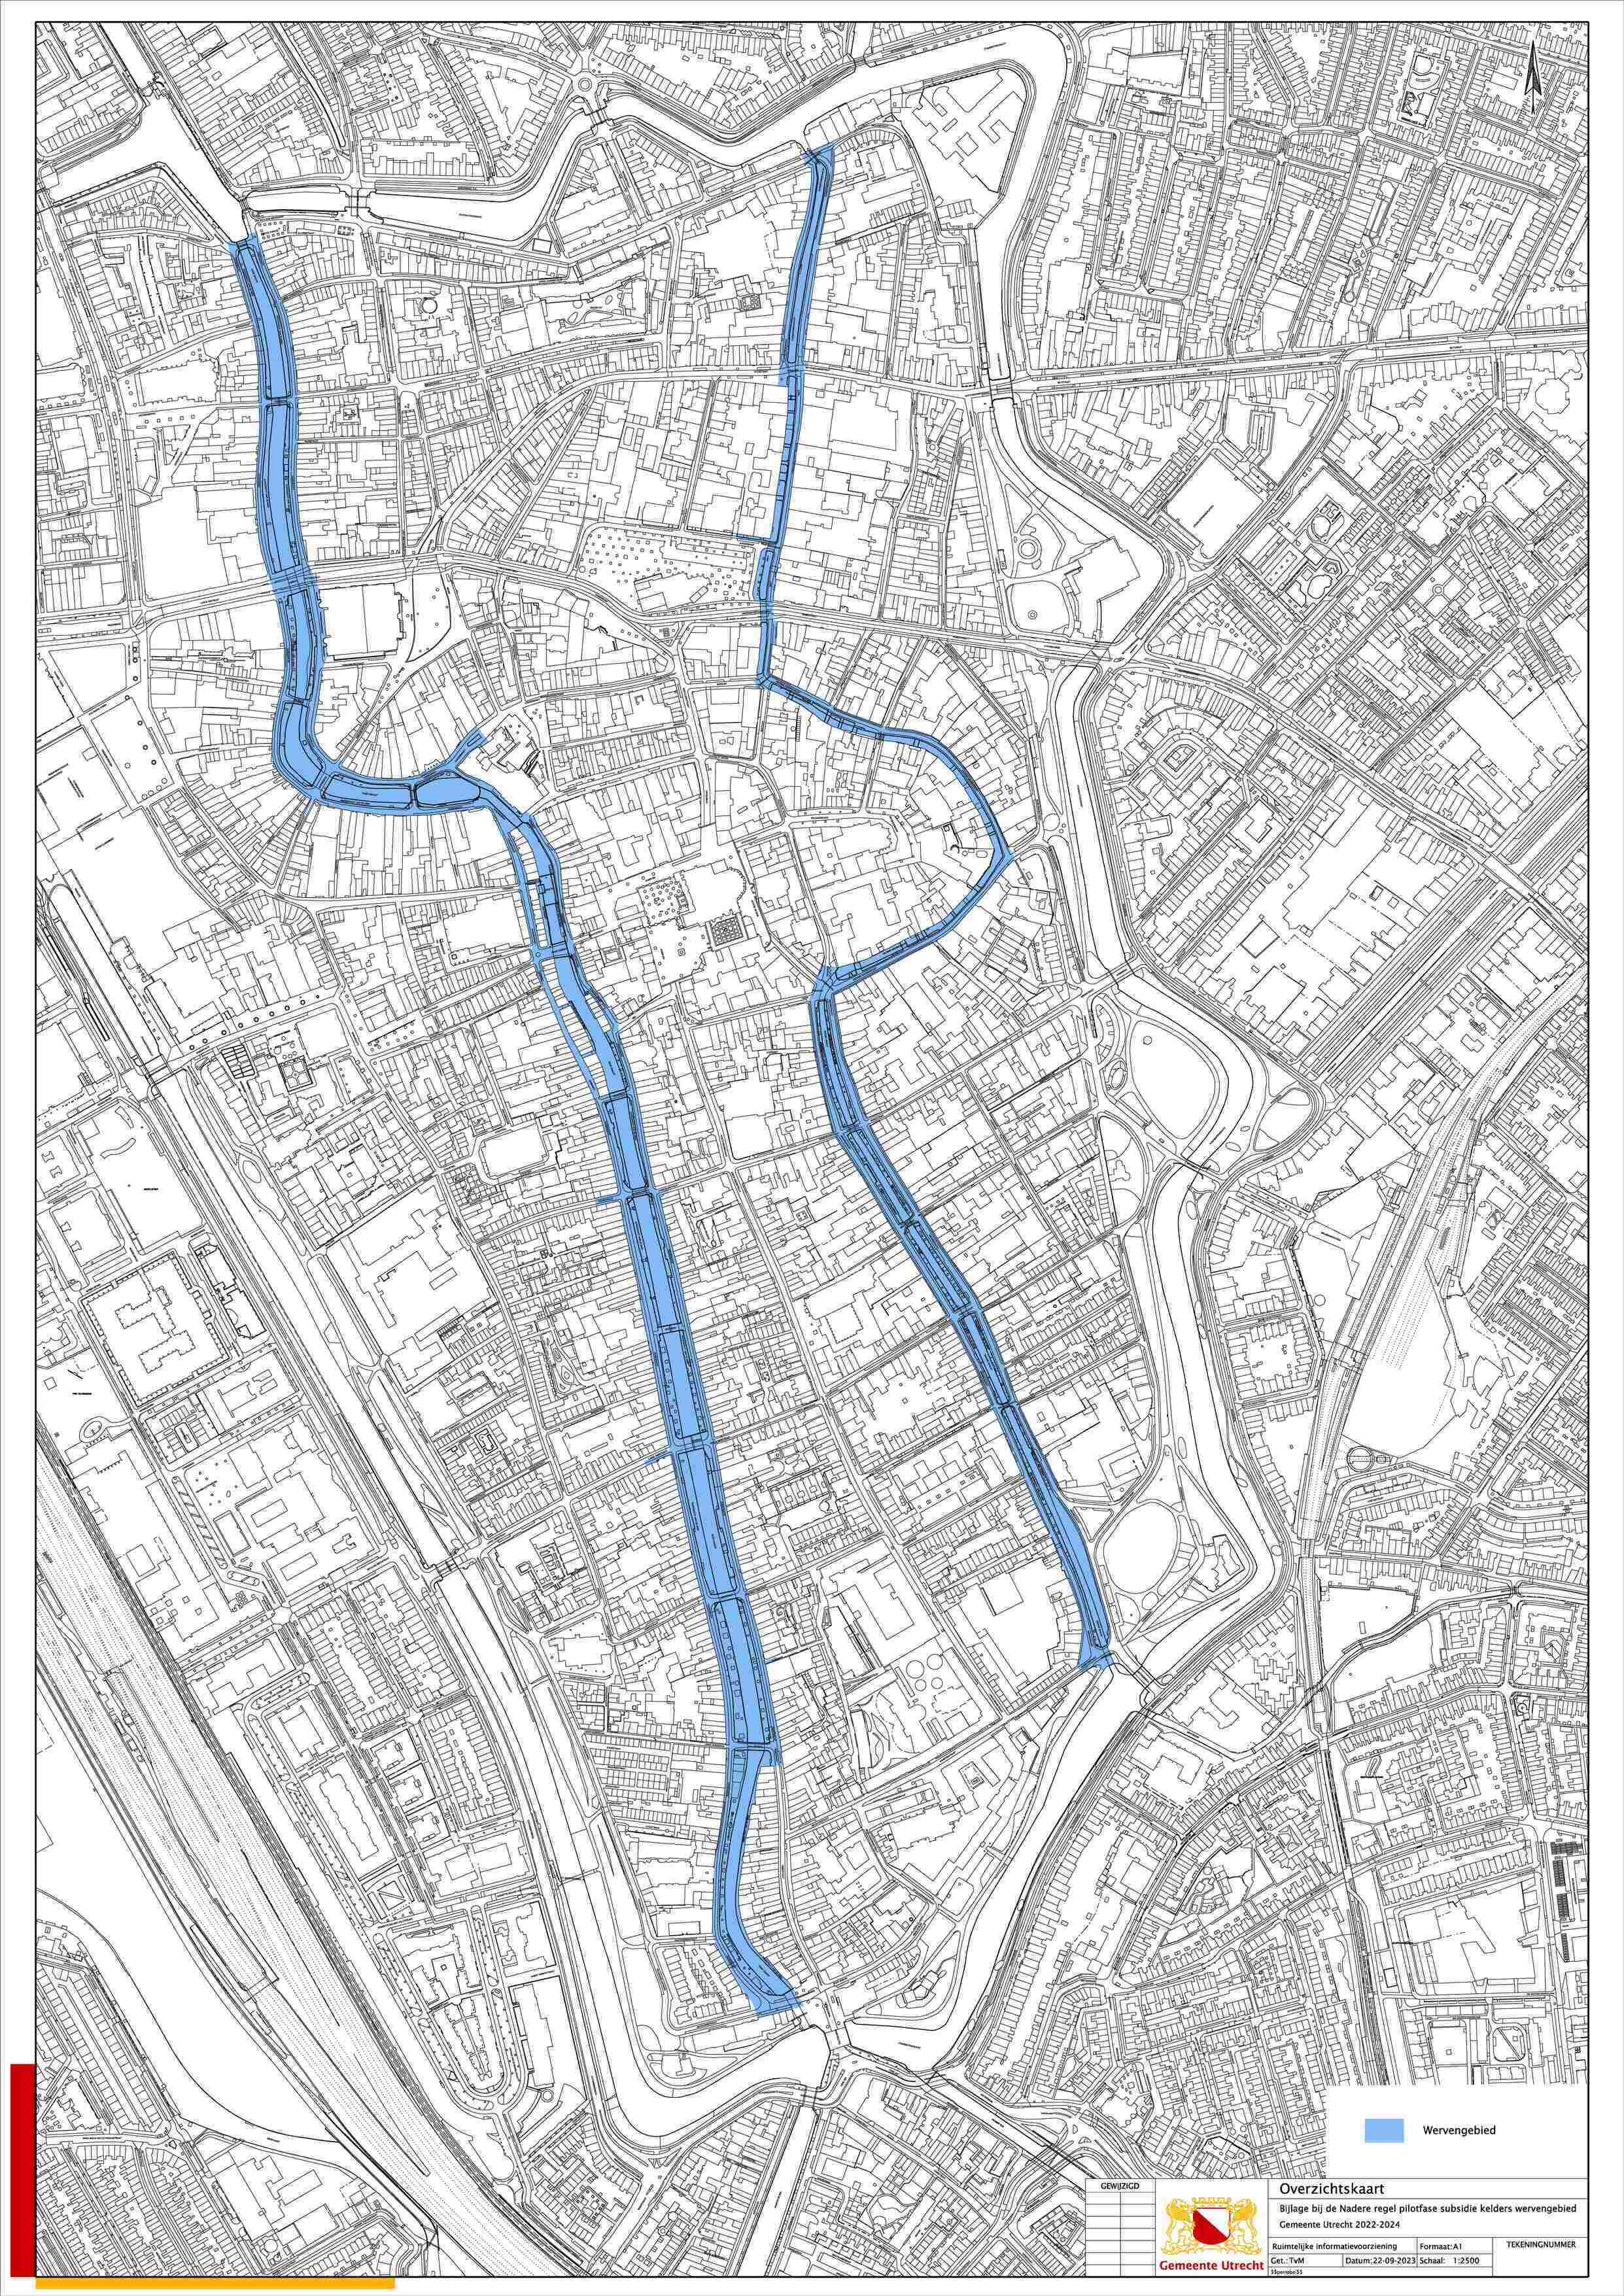
\includegraphics[height=5.0cm]{figures/scope_wervengebiedi83195432-e12f-4974-98be-aaff3c72b58c.jpg}\hspace{2mm}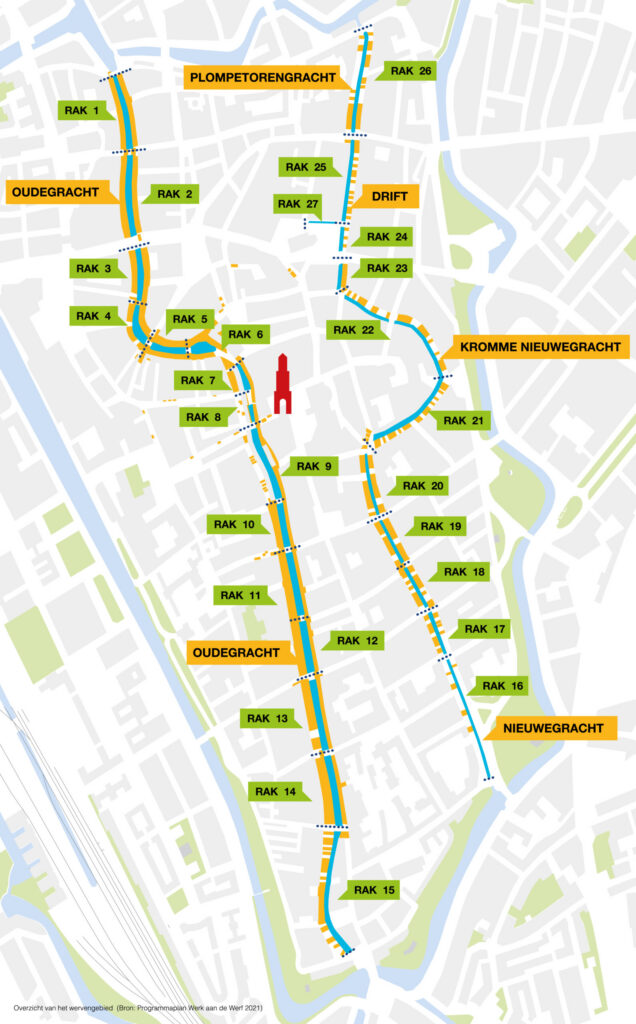
\includegraphics[height=5.0cm]{figures/Plattegrond-wervengebied@2x-scaled-1-636x1024.jpg}
    \captionof{figure}{The Wervengebied: boundary (left) and reaches (\textit{raks}) 1--27 (right). Sources: Gemeente Utrecht (2023); Werk aan de Werf (2021).}
    \label{fig:wervengebied}
    \vspace{-8pt}
\end{wrapfigure}

The Municipality of Utrecht asked our team for a method that supports long-term maintenance decisions for its quay walls. Utrecht has more than 60 km of quay walls and sheet pile walls \parencite{utrecht_teamchallenge2026}. Maintenance is mostly planned on a theoretical end of life, which can differ from the real condition. Money and specialists are limited and the city must stay accessible. Acting too early wastes money. Acting too late is unsafe.

Our goal is a method that sorts quay wall sections by risk and advises a measure (monitoring, restricting use, strengthening or replacement) and an order. It follows the approach of Amsterdam (ARK) and shows where data are missing.

We test the method in the Wervengebied. This is the medieval wharf area along the Oudegracht, Nieuwegracht and Kromme Nieuwegracht (Figure~\ref{fig:wervengebied}). We look at the walls between the water and the wharf. They are about 3.8 km long and divided into 27 reaches (\textit{raks}). Wharf cellars and bridges are left out.

Many of these walls are masonry on timber piles. The city restores about 100~m of wall a year until 2050 \parencite{utrecht_herstelwerven}. Budget and capacity set this pace, not the condition of the walls. The order of work is therefore a real choice.

Inspection can reduce the uncertainty about the wall and the bed level. Traffic, trees, rain and mooring cannot be influenced. Cables, heritage permits and the budget limit the options.

\definecolor{catgreen}{HTML}{4CAF50}
\definecolor{catorange}{HTML}{F59E0B}
\definecolor{catred}{HTML}{DC2626}

\begin{tikzpicture}[
    node distance=12mm and 10mm,
    font=\small\sffamily,
    decision/.style={diamond, aspect=2.2, draw, thick, fill=gray!8,
                     align=center, inner sep=1pt, text width=28mm},
    process/.style={rectangle, rounded corners=2pt, draw, thick, fill=gray!8,
                    align=center, minimum height=9mm, text width=32mm},
    start/.style={rectangle, rounded corners=6pt, draw, thick, fill=gray!20,
                  align=center, minimum height=8mm, text width=30mm},
    category/.style={rectangle, rounded corners=4pt, draw=#1!70!black, thick,
                     fill=#1, text=white, font=\small\sffamily\bfseries,
                     align=center, minimum height=9mm, text width=24mm},
    arrow/.style={-{Stealth[length=2.5mm]}, thick},
    lbl/.style={font=\footnotesize\sffamily, fill=white, inner sep=1.5pt}
]

% Nodes
\node[start] (start) {Quay wall\\ (section)};
\node[decision, below=8mm of start] (life) {Past design\\ life?};
\node[category=catgreen, right=18mm of life] (green) {GREEN};
\node[decision, below=14mm of life] (mas) {Masonry\\ wall?};
\node[category=catorange, right=18mm of mas] (orange1) {ORANGE};
\node[process, below=12mm of mas] (pf) {Calculate failure\\ probability $P_f$};
\node[decision, below=12mm of pf] (thr) {$P_f > P_{f,\mathrm{target}}$?};
\node[category=catred, below left=14mm and 2mm of thr] (red) {RED};
\node[category=catorange, below right=14mm and 2mm of thr] (orange2) {ORANGE};

% Edges
\draw[arrow] (start) -- (life);
\draw[arrow] (life) -- node[lbl] {No} (green);
\draw[arrow] (life) -- node[lbl] {Yes} (mas);
\draw[arrow] (mas) -- node[lbl] {No} (orange1);
\draw[arrow] (mas) -- node[lbl] {Yes} (pf);
\draw[arrow] (pf) -- (thr);
\draw[arrow] (thr.west) -| node[lbl, pos=0.25] {Yes} (red.north);
\draw[arrow] (thr.east) -| node[lbl, pos=0.25] {No} (orange2.north);

\end{tikzpicture}

\newpage
\section{Assumptions, Data Collection and Generation}
\label{sec:assumptions}






The analysis gives a probability of failure $P_f$ and a reliability index
$\beta$ for each walmuur (the low wall between the werf and the canal) that
still stands on its original timber pile foundation. This needs, per wall:
whether the foundation has been renewed, the geometry of wall and foundation,
the retained height, the soil and water behind the wall, the load on the werf
and the condition of the timber piles. The municipal asset register lists the
walls, their length and age, but none of the structural data. We therefore
collected open data and project documents, derived the missing values with
scripts, and filled the remaining gaps with stated assumptions. Within the
time of the project, no data were requested from the municipality.

\subsection{Data collected}\label{sec:data-collected}

Table~\ref{tab:data-sources} lists the data, what each source provides and its
main weakness.

\begin{table}[htbp]
\centering
\small
\caption{Data used for the walmuren, with source and main limitation.}
\label{tab:data-sources}
\begin{tabularx}{\textwidth}{@{}>{\raggedright\arraybackslash}p{2.5cm}
  >{\raggedright\arraybackslash}p{4.3cm}
  >{\raggedright\arraybackslash}X >{\raggedright\arraybackslash}X@{}}
\toprule
Data need & Source & Used for & Limitation \\
\midrule
Walls, length, age & Asset register \cite{gu2025register} & 51 walmuren; screening & No height or foundation data \\
Werf level & AHN 0.5\,m \cite{ahn} & Retained height $H$ & Canal bed not measured \\
Soil & 71 DINO borings \cite{dino} & Soil class, sets $K$ and $\gamma$ & 20--144\,m away; often disagree \\
Groundwater & BRO wells \cite{bro_gmw} & GHG and GLG & Nearest well 143--418\,m \\
Traffic & BGT, NDW \cite{bgt,ndw} & Road distance, axle limit & Road is not on the werf \\
Foundation & Programme reports \cite{antea2019,gu2025up} & Renewed or timber & 8 walls unclear \\
Wall type & TNO dive notes \cite{tno2009} & $P(\text{type 2})$ per rak & Not known per wall \\
Section, piles & \cite{erfgoed156,erfgoed158,ibu2010} & Shapes, levels, piles & Schematic; Oudegracht \\
Timber, method & Hemel \cite{hemel2023,hemel2024} & Pile strength, decay, load & Amsterdam piles \\
Target $\beta$ & NEN 8700 \cite{nen8700} & 1.8 / 2.5 / 3.3 & Class not chosen \\
\bottomrule
\end{tabularx}
\end{table}

The foundation data decide which walls are modelled at all. Of the 51
walmuren, 32 are already renewed on steel, including 11 of the 29 that the
register marks as past their design life. Of the 19 on timber, 2 have no werf:
the street runs to the water, which is a different structure. This leaves 17
walls (611\,m) for the $P_f$ calculation (Appendix~\ref{app:data}).

\subsection{Data generation}\label{sec:data-generated}

Eight scripts turn the raw data into one input row per wall. They run in a
fixed order, each reading the output of the one before
(Appendix~\ref{app:data}). The main generated values are:
\begin{itemize}\setlength{\itemsep}{0pt}\setlength{\parskip}{0pt}
  \item \textbf{Werf level and $H$:} the median of six AHN points on the werf
    side of the wall (+0.99 to +1.57\,m NAP). $H$ is the werf level minus the
    wall underside at $-0.08$\,m NAP \cite{erfgoed158}; median 1.22\,m.
  \item \textbf{Soil class:} the share of clay-like and sand-like soil between
    werf and wall underside in the nearest boring within 250\,m. At least
    70\,\% of one kind gives that class, otherwise ``mixed''. Of the 51 walls,
    23 are clay/peat, 16 sand and 12 mixed.
  \item \textbf{Foundation status:} a hand-compiled table of renewals per rak
    and bank, linked to the register through the city's \emph{Werfmuren} map.
  \item \textbf{Wall type:} divers found a timber beam (\emph{watersloof}, only
    in type 1) or a concrete floor (only in type 2) in some rakken
    \cite{tno2009}, which gives a chance of type 2 per rak.
  \item \textbf{Monte Carlo samples:} 400{,}000 draws per wall and wall type,
    with a fixed seed, for 2026 and 2041 (end of the 15-year reference period
    of NEN 8700).
\end{itemize}
Every raw file is listed with its source and download date, so all results
can be regenerated from the raw data.

\subsection{Assumptions}\label{sec:data-assumptions}
Where no data exist we use the assumptions in Table~\ref{tab:assumptions}.
Uncertain values get a distribution, not a single value. All 27 inputs are
listed in Appendix~\ref{app:data}.

\begin{table}[htbp]
\centering
\small
\caption{Main assumptions where data are missing.}
\label{tab:assumptions}
\begin{tabularx}{\textwidth}{@{}l X l@{}}
\toprule
Quantity & Assumption & Basis \\
\midrule
Canal bed & At the wall underside ($-0.08$\,m NAP), so $H$ is a lower bound & \cite{erfgoed158} \\
Wall type & $P(\text{type 2})$: 0.2 (rak 3--6), 0.5 (rak 21), 0.9 (rak 22), 0.8 (rest) & \cite{tno2009,erfgoed156} \\
Cross-section & Two measured drawings for all walls; floor level $\pm0.15$\,m & \cite{erfgoed156,ibu2010} \\
Pile condition & Soft shell $U(0,45)$\,mm, all walls; grows 0.10--0.25\,mm/yr & \cite{hemel2023} \\
Piles & Diameter $N(180\,\text{mm}, 0.10)$; spacing $U(0.8, 1.2)$\,m & \cite{ibu2010,hemel2023} \\
Soil & $K$ lognormal and $\gamma$ normal per class, independent & Group report, Tab.~C.5 \\
Water & Canal +0.6\,m NAP; groundwater $U(+0.5, +0.9)$\,m NAP & \cite{erfgoed158} \\
Surcharge & $q \sim N(7\,\text{kPa}, 0.20)$ at a distance $U(0,3)$\,m & \cite{hemel2024} \\
Proven strength & Keep only the draws in which the wall stands today & \cite{hemel2024} \\
\bottomrule
\end{tabularx}
\end{table}

\subsection{Effect on the results and validation}\label{sec:data-effect}

The assumptions do not affect the results equally. In order of effect on
$\beta$ (interpreted further in Section~4.2):
\begin{enumerate}\setlength{\itemsep}{0pt}\setlength{\parskip}{0pt}
  \item \textbf{Wall type.} For the same wall, type 1 gives a $\beta$ that is
    1.4--2.4 lower than type 2. With the chance per rak, $\beta$ is 0.1--1.5,
    so all 17 walls are below 1.8. If all were type 2, 7 of the 17 would pass
    1.8. Whether a wall passes therefore depends mostly on its type, which the
    original drawings or a dive inspection can settle.
  \item \textbf{Pile condition.} For type 2 the piles fail far more often than
    the wall overturns (median $P_f$ 0.075 against 0.004). The same broad
    shell is used for every wall, so it shifts all $P_f$ but not the ranking.
  \item \textbf{Retained height and soil.} The soil moment grows with $H^3$:
    0.1\,m more height adds about 25\,\%. As $H$ is a lower bound, this
    assumption makes $P_f$ too low. Clay/peat gives 43\,\% more soil load than
    sand, and nearby borings agree for only 9 of the 51 walls.
  \item \textbf{Surcharge.} 7\,kPa is heavy for a pedestrian werf, so this
    assumption makes $P_f$ too high.
\end{enumerate}

We checked the data and assumptions where possible. The median AHN werf level
on the Oudegracht (+1.13\,m NAP) matches the +0.95 to +1.15\,m NAP measured in
\cite{erfgoed156,erfgoed158}. The renewed length in our foundation table
(about 3.36\,km) matches the city's 3{,}356\,m. The strongest check is that all
17 walls stand today. A first model that treated the wall as a masonry block
gave $P_f \approx 1$ and was rejected. With the measured sections, a type-2
wall stands in 87--100\,\% of the draws, a type-1 wall in only 10--98\,\%.
Either the type-1 model is conservative or many of these walls are type 2; the
proven-strength update accounts for this.

Settlement from pile rot, the damage actually seen on these walls
\cite{erfgoed156}, and failure of the timber screen are not modelled. The
$\beta$ values should therefore be read as an indicative ranking and order of
magnitude, not as exact values. The data that would improve them most are the
wall type per wall, the measured pile condition and canal soundings.


%% ----------------------------------------------------------------------
%%  MAX 2 PAGES  |  RUBRIC WEIGHT 10%
%%
%%  TASK DESCRIPTION
%%  Describe and represent the needed data and how it is relevant to the
%%  problem identified in Section \ref{sec:problem-synthesis}. You may
%%  consider references in data records, literature, or stakeholder
%%  elicitation.
%%  Generate other data that you need. Explain the process and the input
%%  data to guarantee reproducibility of your results.
%%  Indicate sound assumptions to support the problem analysis when data
%%  is not available.
%%  Link to the interpretation of the results in Section
%%  \ref{sec:results-recommendations} and reflect on to what extent the
%%  lack of data accuracy or the uncertainty associated with the data
%%  assumptions may impact your analysis and results. Discuss and validate
%%  the use of the assumptions in the analysis.
%%  This section provides an overview. Use the appendices for supporting
%%  information.
%%
%%  CHECKLIST (challenge task 2: assemble the evidence and confront theory
%%  with observed performance)
%%   - Build a small structured dataset of the assets in your scope from
%%     public sources, and document its provenance, completeness and known
%%     errors. A data quality table is often more informative than the
%%     data itself.
%%   - Exploit proxy data: satellite-based deformation from the
%%     bodemdalingskaart, groundwater levels from the BRO, tree registers,
%%     traffic counts, dredging and water-level records, street-level
%%     imagery over time.
%%   - Take one asset and contrast its code-based assessment outcome with
%%     its observed service history; state what the discrepancy implies
%%     for the rest of the portfolio.
%%   - Consider inspection and monitoring records, field and proof
%%     testing, documented failures elsewhere, and the 'proven strength'
%%     implied by decades of survival under load.
%%   - Reflect on how the gaps in this evidence limit what you can
%%     conclude.
%%
%%  NOTE: the team may submit ONE concrete and justified data request to
%%  the Municipality of Utrecht through the teaching team. Provision is
%%  not guaranteed, so the analysis must also work without it.
%% ----------------------------------------------------------------------


\section{Problem Exploration and Dimension Reduction}

\label{sec:dimension-reduction}

%% ----------------------------------------------------------------------
%%  MAX 1.5 PAGES  |  RUBRIC WEIGHT 5%
%%
%%  TASK DESCRIPTION
%%  Identify the variables playing a role in your problem and analyse how
%%  their levels of variability and uncertainty might affect the final
%%  result.
%%  Reflect on the results. For example: to what extent does a specific
%%  variable really change the results? Do the results correspond to your   
%%  beliefs? How does the lack of accuracy of the data you use affect the
%%  results? Which datasets require more attention, and which estimations
%%  can be made without a significant loss of credibility in the
%%  conclusion?
%%  Decide which variables deserve more effort to reduce their variability
%%  and indicate those whose variability can be neglected.
%%  Justify the process and the use of specific tools for the analysis.
%%
%%  CHECKLIST (challenge task 3: establish which variables drive the
%%  outcome)
%%   - Run a sensitivity analysis and be clear about what your chosen
%%     method can tell you.
%%   - Reduce the problem deliberately: fix variables at defensible
%%     values, aggregate assets into homogeneous classes, or represent a
%%     stretch by a few characteristic cross-sections. Justify each
%%     reduction and estimate what accuracy it costs.
%%   - Turn the result into an inspection strategy: which measurement
%%     would most reduce the variance of your output, and on which assets?
%%     This is the municipality's own question, given more than 60 km of
%%     structures and a limited inspection budget.
%% ----------------------------------------------------------------------


We screen inputs on three outputs: Pf, P(red) and the rank of the 27 reaches Pf is continuous and suited to variance-based indices; the class and rank are discrete, so there we test how many reaches change class when an assumption (A2,A4,A6) is varied. Variables with a total-order index below x are fixed at a defensible value; the remaining n variables are carried as random variables in chapter 2.


Screening variables (determine green/orange): 

- year of construction or last restoration, hence age - asset inventory, available

- design life (100 year, A2) - assumption

- wall type / material (masonry or not) - asset inventory

- foundation type (timber piles, A4) - assumption


Variables for the failure probability Pf (only masonry beyond design life):

- pile diameter - literature value

- decay rate - literature value

- timber strength - literature value

- load (traffic/surface) - literature and traffic data

- groundwater level - nearest BRO well

-soil and surface characteristics - PDOK, BRO


tornado method 


The performance of quay walls and other retaining structures are largely influenced by a number of structural, environmental and demand. This section breaks down the key variables determining the life of quay walls in Utrecht and thus governing the programming of their maintenance. It outlines the influence of the variables on the decisions about the inspection and scheduling of the required intervention, based on their levels of uncertainty in data availability and reasonable assumptions as described in section 1.2.
The aim is to reduce complex asset management programming into a set of measurable variables whose weights and probabilistic projections inform risk of failure by extension aid in scheduling of intervention works. The outlined variables therefore form the basis for the probability calculations and subsequent risk analysis to quantify the likelihood and consequences of potential failure and used to prioritise appropriate maintenance interventions.
The variables were selected based on their theoretical relevance to the structural performance of quay walls, evidence from previous studies and expected influence on failure. The selection was also constrained by the availability of existing data as well as the monetary and time requirements associated with obtaining additional information through testing.

\subsubsection{Design loads}

For comprehensive asset management, it is imperative to identify the loads the structure was designed to bear so as to provide a reference for determining the capacity and subsequently safety in use and assess potential failure. In the analysis of Utrecht quay walls, the design loads are a key demand variable against which current and projected loads up to 2050 are compared.
The design load establishes the range of demand that the structure was intended to accommodate within its theoretical design life. A key uncertainty is the factor of safety incorporated in the original design and its relationship with the safety requirements related to actual loading. Rather than assuming that the historical factor of safety remains directly applicable, sensitivity analysis can examine how reducing or varying the original safety margin affects the assessed structural capacity. The historical design demand can therefore be compared with the corresponding resistance under different safety factors. The factors of safety used in the original design, where available or reasonably estimated, are used to determine the relationship between the specified design demand and the theoretical load-bearing capacity. The resulting range between the original design load and the theoretical maximum at the end of life provides the basis for assessing how changes in demand may influence the probability and timing of failure.


\subsubsection{Traffic Loading}

The loads applied to quay walls over their service life include permanent loads from the self-weight of the structure and earth pressure from retained soil, together with variable loads such as wind, water-current and traffic loads. Traffic loading is associated with relatively high uncertainty because it varies with traffic volume, vehicle composition and changes in demand over time. For uniform analysis, traffic demand is characterised using annual average daily traffic (AADT), while national vehicle-weight data are used to estimate peak traffic loading.
Traffic loading is not treated as the total loading condition of the quay wall and is therefore not directly assessed against the total design load as an isolated variable. Instead, its uncertainty and relationship with the overall structural capacity are modelled to determine its contribution to the probability of failure. Sensitivity analysis assesses how changes in traffic loading influence this probability. Future traffic demand is projected to 2050 and beyond using both annual and local traffic-growth rates, allowing the relationship between increasing traffic demand and available structural capacity to be examined over time. This provides a basis for assessing whether traffic access restrictions could reduce the probability of structural failure in future.


\subsubsection{Soil Type}

The type of soil influences quay-wall behaviour through its geotechnical properties that can influence deformation and structural behaviour such as differential settlement due to variations in ground behaviour. The analysis considers soil type with reference to expansive behaviour that informs consolidation and wetting and drying effects on strength. These are best estimated based on the relation with measurable soil properties of density, cohesion and friction angle.
Expansive soils undergo volume changes with variations in moisture which alter soil properties. Consolidation can result in progressive settlement under sustained loading, potentially contributing to differential movement. These ground responses are to assess how changes in soil behaviour affect the response of the quay wall.
For dimension reduction, sensitivity analysis is used to determine the extent to which uncertainty in soil characteristics and behaviour influences the predicted structural response and failure probability. 


\subsubsection{Structural Material}

Material type is a key variable because the quay-wall portfolio comprises different structural materials, principally timber, steel, concrete and masonry, each with different deterioration mechanisms and rates. Material therefore influences the expected development of structural condition and the remaining capacity of the asset over its service life.

The deterioration rate of each material is considered in relation to the environmental conditions to which it is exposed. In particular, wetting and drying and groundwater conditions may influence the rate and nature of material deterioration. The deterioration process is treated as an uncertain variable because the actual condition and rate of deterioration are not readily measurable across the entire portfolio and may vary between structures and exposure conditions.
For dimension reduction, material type is used to establish the expected deterioration behaviour, while the uncertainty in deterioration rate and current condition is incorporated into the assessment. Sensitivity analysis can determine whether differences in deterioration assumptions materially affect the predicted structural performance and failure probability, thereby identifying where further inspection or material-condition data would have the greatest value for maintenance programming.


\subsubsection{Type of Foundation}

The type of foundation is a significant variable in the assessment because it determines the mechanism through which structural loads are transferred to the ground and therefore influences stability. Shallow foundations are more dependent on near-surface soil and groundwater characteristics, while deep foundations can provide greater stability where shallow conditions are unsuitable, although their condition and behaviour are harder to verify.
In the probabilistic model, uncertain properties of condition and settlement response are represented through probability distributions and their dependence on soil and groundwater conditions. Sensitivity analysis can then establish whether foundation-related uncertainty materially affects predicted stability and failure probability and consequently maintenance decisions. Where sensitivity is high, geotechnical investigation should be prioritised else the variable can be simplified without reducing the credibility of the model.


\subsubsection{Previous Maintenance Records}

Previous maintenance records are an important variable because they provide evidence of how a structure has performed, deteriorated and been repaired over time. Historical records can therefore contribute to estimating remaining service life, deterioration rates and the probability that maintenance will be required within a given planning period. In a probabilistic programming model, this information is used to update the probability of failure rather than just using age of the structure to determine remaining structural life, contributing to the confidence of the intervention timelines and procedures.


\subsubsection{Significance of variables}

Not all variables identified above contribute equaly in the final failure probability. Chapter~\ref{chapter:probabilistic-modelling} shows that pile diameter has the greatest influence in the model, with an influence coefficient $\alpha^2$ of 0.73, against 0.14 for soil and 0.06 for surface load (Appendix~\ref{app:pm-calibration}). Thus, pile geometry is the dominant physical variable, while soil uncertainty remains relevant and surface load has a smaller direct influence. Assumption A1 and foundation type are also important at the portfolio level, although foundation type is not quantified directly in the current timber-pile model.

\textbf{Soil Type} and groundwater conditions are significant mainly through their effect on deterioration rather than through the load directly: Section~\ref{sec:probabilistic-models} shows that a dry groundwater regime lowers the reliability index $\beta$ from 1.41 (moderate) to 0.93, and to 0.81 under the KNMI'23 climate shift, because fungal decay becomes active in a much larger share of samples. \textbf{Structural Material} is significant at the scope level rather than within the current model: the timber-pile mechanism analysed here does not apply to the steel and concrete sections elsewhere in the portfolio (Assumption~A12), so material type determines which model applies before it can influence any single failure probability.

\textbf{Previous Maintenance Records} are significant less for the base failure probability and more for how much that probability can be revised: Section~\ref{sec:probabilistic-models} shows that survival of a known load raises $\beta$ at the moderate location from 1.41 to 2.22, a larger shift than most of the modelling assumptions produce on their own. Variables with little direct influence on the ranking, are fixed at a defensible value rather than treated as a full random variable, since this does not materially change the result.


%\subsubsection{Sensitivity Analysis}Two complementary tools are used: a tornado analysis first screens the candidate variables to remove those with negligible influence, so that computational effort is spent on the ones that matter. The influence coefficients reported in Appendix C.1 are estimated from the standardised input values in the simulated failure samples.This analysis is applied at two levels. At the level of a single section, it identifies which physical variable a measurement should target first: since pile diameter carries by far the largest share of the variance, Section~\ref{sec:probabilistic-models} concludes that a direct diameter measurement is worth more than a refined soil model. At the level of the assumptions themselves, the same logic is applied to A1, A2 and A5 (Section~\ref{sec:data-quality}): each is varied within its stated range, and the resulting change in $\beta$ and in the section ranking is compared against the change produced by the physical variables. Where an assumption shifts the ranking by as much as, or more than, a genuine physical variable, it is flagged as a priority for the municipality's data request rather than left as a fixed input.The three groundwater scenarios in Figure~\ref{fig:pm-results}a are a direct product of this analysis: they were selected because groundwater level drives both the load path (through $k_w$) and the deterioration path (through fungal decay), so its effect could not be adequately summarised by a single sensitivity coefficient and is instead shown as a full scenario comparison.\subsubsection{Justification of Analysis Tools}



\section{Approach Selection}
\label{sec:approach-selection}


The approach is a coarse-to-fine screening of the quay-wall sections, shown in \hyperlink{figure.caption.5}{Figure~1.2}. It is based on the Amsterdam ARK method~\cite{ark2023}. Cheap rules based on the asset register sort the whole portfolio first. The expensive probabilistic analysis is used only where it can change a decision. This suits the problem in \hyperlink{section.1.1}{Section~1.1}. Utrecht holds basic asset data for every section, such as construction year, restoration year and wall type. It does not hold foundation data, pile dimensions or design calculations for the Wervengebied (\hyperlink{section.1.2}{Section~1.2}). Running a detailed deterministic recalculation of all 27 reaches is therefore not possible with the data we have. A purely qualitative ARK score would also fall short, because it does not quantify uncertainty.

\paragraph{Step 1 -- Rule-based screening.}
The theoretical end of life of each section is the year of construction or last full restoration plus a design life of 100 years (A2). If this falls after 2030, the section is classified green and goes into regular maintenance (A3). We chose 2030 because that is when the municipal inspection programme ends~\cite{utrecht_teamchallenge2026}. Sections that reach their end of life by 2030 are then screened on material. Non-masonry walls are classified orange: their deterioration (corrosion, concrete degradation) needs a different model and further inspection. Masonry walls on timber piles (A4) go on to Step~2. This is the most common typology in the scope, and its capacity is the most variable and the least well documented.

\paragraph{Step 2 -- Probabilistic failure model.}
For masonry walls, the failure probability $P_f$ of lateral foundation failure is calculated over the 15-year reference period of NEN~8700~\cite{nen8700} (\hyperlink{chapter.2}{Chapter~2}). We use crude Monte Carlo simulation ($n = 10^6$) instead of FORM, for four reasons:
\begin{itemize}
    \item the limit state is strongly non-linear in the pile diameter;
    \item fungal decay enters through yearly indicator functions of the groundwater level;
    \item dependence between adjacent sections can be imposed directly with a Gaussian copula;
    \item updating with past performance (proven strength) only requires filtering the surviving samples~\cite{hemel2024}.
\end{itemize}
At the $P_f$ levels we are interested in ($10^{-2}$--$10^{-1}$), the computational cost is small. Influence coefficients are estimated from the Monte Carlo design point. We do not have the original pile-group model, so a response function calibrated to Hemel et al.~\cite{hemel2024} replaces it. Because of this, $P_f$ is used to compare sections and scenarios, not as an absolute value.

\paragraph{Step 3 -- Sensitivity analysis and dimension reduction.}
Before the model is applied to all reaches, we screen the inputs (\hyperlink{section.1.3}{Section~1.3}). For the continuous output $P_f$, influence coefficients and scenario runs show which variables matter. Pile diameter dominates, with $\alpha^2 = 0.73$; groundwater acts through decay. For the discrete outputs (class and rank), we use a tornado-type analysis on the assumptions A2, A4 and A6, and count how many reaches change class. Variables with little influence are fixed. Variables with high influence become priorities for inspection, which also informs our data request.

\paragraph{Step 4 -- Consequences and risk classification.}
Consequence indicators are scored from 1 to 4 on the ARK scales (A7)~\cite{ark2023}: traffic function, trees, adjacent buildings and cellars, and quay use. These scores are combined into a consequence score $C$ with explicit weights. Where municipal priorities are unknown, the weights are treated as value judgements and varied in the sensitivity analysis. The consequence level sets the NEN~8700 consequence class. A section is red when $P_f$ exceeds the limit for its class (A6), and orange otherwise. Within each class, sections are ordered by the relative risk $R = P_f \cdot C$.

\paragraph{Step 5 -- Uncertainty in the ranking.}
The uncertain inputs and weights are propagated through the whole procedure, with the same rules applied to every section in each run. The output is therefore a distribution, not a single list: the probability that a reach is red, $P(\text{red})$, its rank distribution, and the probability that one reach outranks another. Assumptions that apply equally to all walls shift every $P_f$ in the same direction, so the ordering is more robust than the absolute values.

\paragraph{Link to the following chapters.}
The red and orange sections feed into the fault tree (\hyperlink{section.3.1}{Section~3.1}). There, structural failure is one causal path next to human and organisational causes of programme failure. The decision tree (\hyperlink{section.3.2}{Section~3.2}) compares interventions for these sections: monitoring, restricting use, strengthening and replacement. Regression (\hyperlink{section.4.1}{Section~4.1}) extrapolates the backlog and risk exposure towards 2050 for different production rates.

% --- Hieronder jullie bestaande figuurcode voor Figure 1.2 laten staan ---


Red: the condition looks so poor that the probability or consequence of failure is too high. This means intensive monitoring and fast follow-up.

Orange: the condition is still unknown and more investigation is needed.

Green: the structure can carry its current use, so regular maintenance is enough.

The steps are:

\begin{enumerate}
    \item Beheerdersoordeel (the asset manager's judgement): a first classification based on limited data.
    \item ARK (Amsterdamse Risicobeoordeling Kademuren): a qualitative risk assessment for orange walls, based on inspections, archives and diver reports. It is done in Excel, and external experts give second opinions.
    \item Herberekening (recalculation) under TAK: for orange walls, the city first decides whether a recalculation is worth it, because it costs a lot of time, money and capacity.
    \item Verfijnd toetsen (refined assessment) under TAK: a more detailed analysis of specific elements.
    \item Integrated management advice for red walls: technical advice is combined with the impact on the surroundings to choose a measure.
    \item Green walls: these go into regular maintenance planning.
\end{enumerate}




The objective is to categorise Utrecht’s quay walls according to their risk of failure, supporting the prioritisation of inspections and maintenance under limited resources. A coarse-to-fine screening approach is adopted, combining rule-based screening with probabilistic analysis. This is suitable because the available asset records and historical inspections provide useful initial information, but incomplete design loads, foundation records and material properties limit the feasibility of detailed deterministic assessment of every structure.

For the initial screening, the theoretical end-of-life year is considered first. Structures with an end-of-life year after 2030 are classified as green, based on the assumption that they are relatively safe and less critical within the study horizon. Structures reaching their theoretical end of life by 2030 proceed to material screening. Masonry structures proceed to detailed analysis while non-masonry structures, including concrete and steel structures, are classified as orange for further inspection. Concrete generally offers higher compressive strength than unreinforced masonry, whose resistance depends on unit and mortar properties (NEN-EN 1996-1-1:2025), while steel has high tensile strength. However, structural capacity depends on capacity and deterioration can lead to loss of strength thus causing uncertainty in materials properties. Masonry structures require immediate in-depth analysis due to their lower and more variable capacity, combined with deterioration-driven loss of strength, creates the greatest uncertainty in structural performance (Materials and Structures,2022).


A probabilistic multi-criteria prioritisation model is selected to rank quay-wall sections by relative risk and assessment urgency.This approach suits the incomplete, heterogeneous information available and provides a reproducible basis for comparing additional sections. An assumption that you apply in the same way to every wall shifts all failure probabilities in the same direction and largely preserves the ordering. That's why the ordering is a robus approach

The technical variables identified in the preceding sections provide inputs to the probabilistic failure model described in Chapter~3. Their effects are represented through the relationships between loading, deterioration and structural resistance, with uncertain inputs described by probability distributions where appropriate. Input assumptions, sources and dependencies will be documented. Consequence indicators will be defined to represent the potential impacts of failure and normalised to a common scale using explicit, justified reference values.

The normalised consequence indicators will be combined using an explicit weighting scheme to obtain a consequence score \(C\). This score will be combined with the model-based failure probability \(P_f\) to calculate a relative risk score, \(R = P_f \times C\), for prioritising quay-wall sections. Literature and relevant guidance will inform the selection and scaling of consequence indicators. The weights will reflect municipal priorities where these can be established; otherwise, they will be documented as value judgements and varied in sensitivity analysis to assess their influence on the ranking.

Monte Carlo simulation propagates uncertainty in inputs and weights through the ranking procedure while preserving specified dependencies. Each run applies common scoring rules and weights to all compared sections. Outputs include score uncertainty, rank distributions and the probability that one section outranks another, conditional on the adopted assumptions.

Global sensitivity analysis will identify which inputs influence the ranking. The results will guide the identification of less influential variables and indicate where additional inspection or data collection could improve confidence in the prioritisation. Assessment of loading variables will also inform the operational interventions considered in the subsequent trade-off analysis.




\begin{figure}[htp]
    \centering
    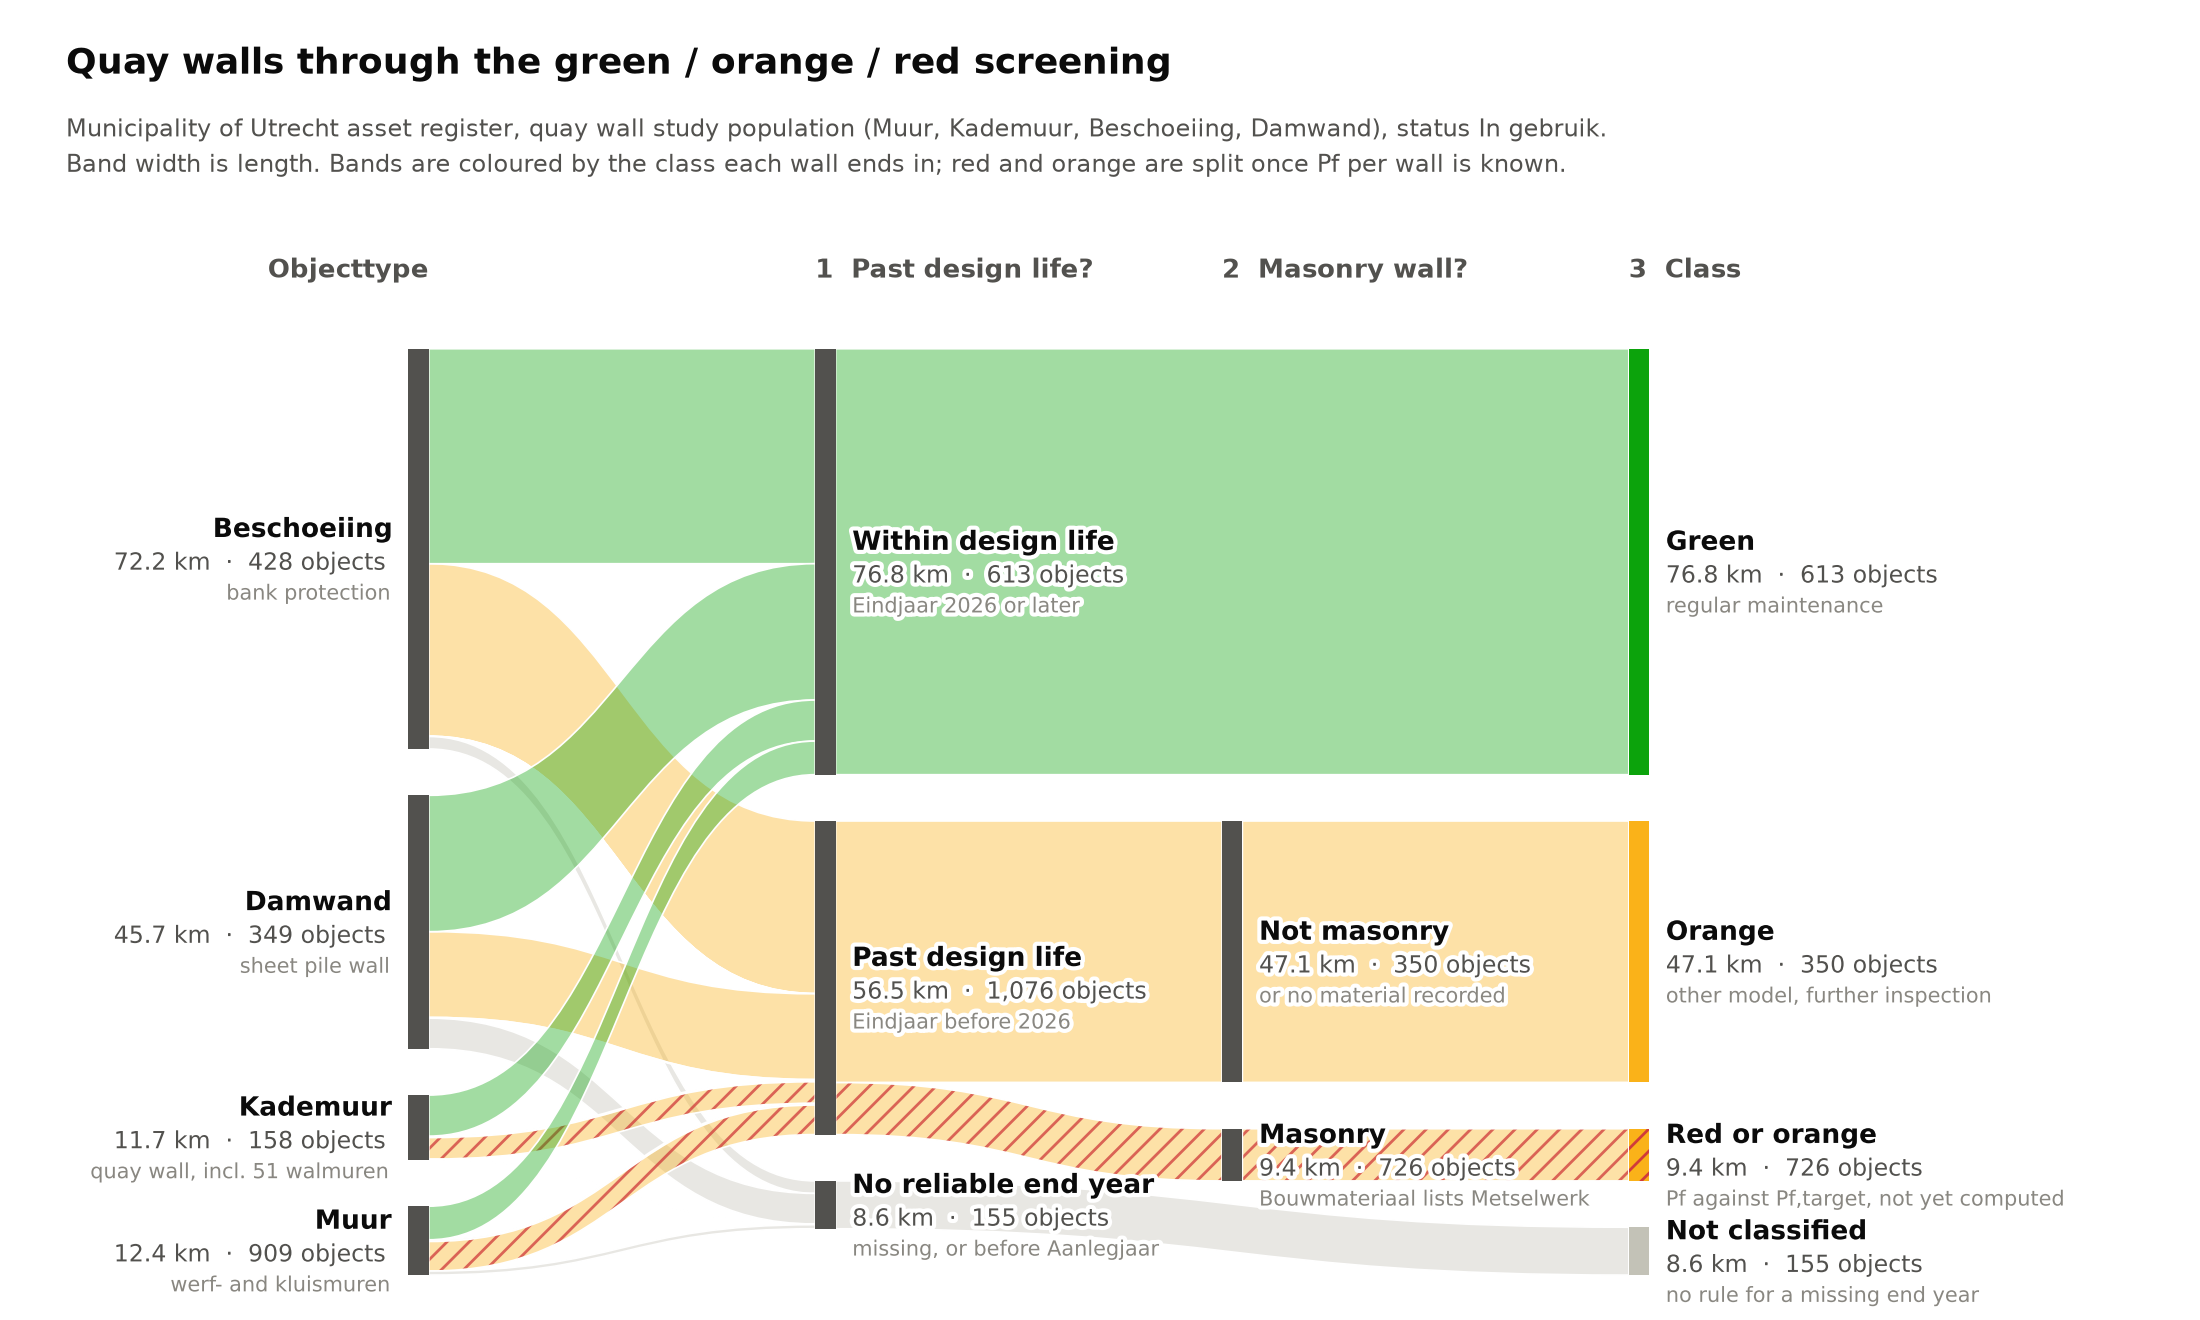
\includegraphics[width=0.75\linewidth]{figures/screening_sankey_register.png}
    \caption{Scoping of the selected area}
    \label{fig:placeholder}
\end{figure}


%% ----------------------------------------------------------------------
%%  MAX 1 PAGE
%%
%%  TASK DESCRIPTION
%%  Explain or represent the approach you will follow to achieve your
%%  goal. You can use a flowchart or graphical representation to convey
%%  the main idea. You can provide both the general picture and a detailed
%%  description of the tools and methods, avoiding definitions of the
%%  methods or other trivial information.

%%  Motivate what modelling tools and uncertainty quantification methods
%%  you choose for the analysis and why. You may compare relevant tools
%%  learned in the course and choose the adequate ones considering the
%%  defined problem and the available data.
%%
%%  NOTE: the challenge tasks are examples, not requirements. If the team
%%  addresses only some of them or takes a different route, that choice
%%  must be justified here.
%% ----------------------------------------------------------------------

